\chapter{Análisis Exploratorio de los Datos (EDA). Dataset de clasificación: Bupa}

\section{Descripción del dataset: Bupa}
El dataset \textbf{Bupa} contiene los resultados de diferentes tipos de análisis de sangre sensibles a los trastornos hepáticos que pueden surgir con un consumo excesivo de alcohol. Datos donados en el 1990. Cada fila de este conjunto de datos contiene el registro de un solo individuo masculino. \cite{5} \\

Un dato importante de este conjunto de datos, es que la séptima variable solía malinterpretarse como una variable que indica la presencia o ausencia de un trastorno hepático, pero esto es incorrecto, esta variable fue creada por investigadores para separar los datos en un conjunto de entrenamiento y otro de test.\\

Teniendo en cuenta la función de esta séptima variable, este dataset está formado por 5 variables independientes, las cuales corresponden a los resultados de diferentes análisis de sangre y una variable dependiente, todas variables numéricas. Se recogen un total de 345 muestras que representan el registro de cada individuo masculino.
Se presentan a continuación las variables independientes:
\begin{itemize}
	\item \textbf{mcv}: Variable numérica real que refleja el volumen corpuscular medio
	
	\item \textbf{alkphos}: Variable numérica real que refleja la fosfatasa alcalina, una enzima responsable de eliminar grupos de fosfatos de varios tipos de moléculas como nucleótidos, proteínas y otros compuestos fosforilados. Los niveles de fosfatasa alcalina elevados podrían ser signo de daño en el hígado.
	
	\item \textbf{sgpt}: Variable numérica real que refleja la alanina aminotransferasa, enzima que se encuentra principalmente en las células del hígado. Niveles altos de esta puede indicar que tiene algún tipo de daño en el hígado. 
	
	\item \textbf{sgot}: Variable numérica real que refleja la aspartato aminotransferasa, otra enzima del hígado. Los niveles elevados de esta en la sangre pueden indicar hepatitis, cirrosis, mononucleosis u otras enfermedades del hígado
	
	\item \textbf{gammagt}: Variable numérica real que refleja la gamma-glutamil transpeptidasa, es una enzima hepática. Se mide su nivel en sangre siendo un marcador de laboratorio de enfermedad hepática (mala en altos niveles).
	
	\item \textbf{selector}: Variable numérica entera creada por los investigadores para dividir los datos en el conjunto de train y test. 
\end{itemize}

La variable dependiente utilizada para la clasificación es \textbf{drinks}, un valor numérico real que refleja el número de medias pintas equivalentes a la cantidad de bebidas alcohólicas que se beben por día. 


\vspace{1cm}
\section{Planteamiento de hipótesis}
\begin{itemize}
	\item \textbf{Una mayor masa corporal puede dar lugar a casos en los que un alto consumo de alcohol no se vincule con altos resultados en los análisis de sangre.}
	\item \textbf{¿Un valor alto en uno de los test de análisis de sangre equivale a un valor alto en el resto de test?}	
	
\end{itemize}




\vspace{1cm}
\section{Procesamiento de los datos}
Siguiendo la misma idea que con el dataset anterior se pretende profundizar en los diferentes atributos que componen este conjunto de datos para ampliar el conocimiento sobre este y determinar cualquier característica que facilite el posterior desarrollo de modelos. \\

El primer paso es la búsqueda de valores perdidos dentro de los datos, concluyendo en que este dataset no posee ningún Missing value.
Sin embargo se detectan 4 filas duplicadas, las cuales procedemos a eliminar, reduciéndose el número de muestras a 341.




\newpage
\subsection{Análisis de las variables independientes}\label{anali}
Se analiza el comportamiento de las diferentes variables mediante el calculo de diversas medidas de posición: la media aritmética, mediana, primer y tercer cuartil, valores máximos y mínimos de cada variable. También se estudia la dispersión de las distribuciones mediante el calculo  de la desviación típica, mientras que la normalidad de los datos se estudia con los coeficientes de Skewness y Kurtosis.

Se estudia cada variable en detalle mediante el calculo de las medidas previamente mencionadas. Dicho estudio es acompañado con una serie de representaciones gráficas que facilite la comprensión de los resultados:

\begin{itemize}
	\item \textbf{mcv}
	\begin{table}[h!]
		\centering
		\begin{tabular}{ll}
			& mcv        \\
			Valor mínimo            & 65.00      \\
			Primer cuartil          & 87.00      \\
			Mediana                 & 90.00      \\
			Media                   & 90.12      \\
			Tercer cuartil          & 92.00      \\
			Valor máximo            & 103.00     \\ \hline
			Desviación estandar     & 4.4523855  \\ \hline
			Coeficiente de skewness & -0.3765269 \\
			Coeficiente de Kurtosis & 5.542126  
		\end{tabular}
	\end{table}
	
Se presenta una variable con un rango de valores definidos entre [65, 103]. Con un centro de distribución muy levemente desplazado a la derecha, se presenta una leve dispersión de los datos respecto a este centro de dispersión.
Se profunda la información mediante un diagrama boxplot y un histograma:
\begin{figure}[h!]
	\centering
	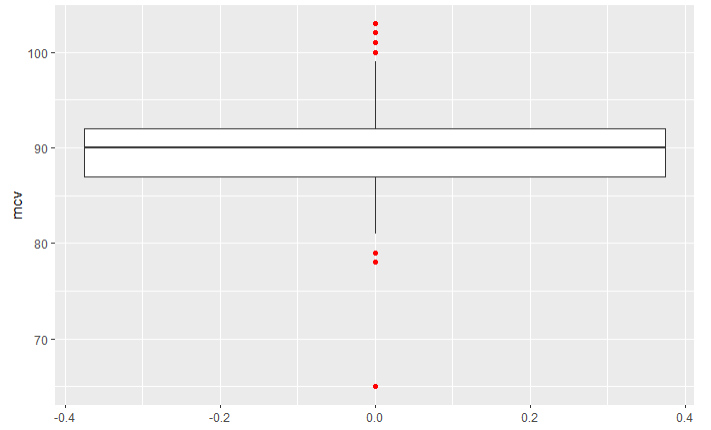
\includegraphics[width=0.7\linewidth]{figures/box_1}
	\caption{Diagrama de cajas mcv}
	\label{fig:box1}
\end{figure}

\begin{figure}[h!]
	\centering
	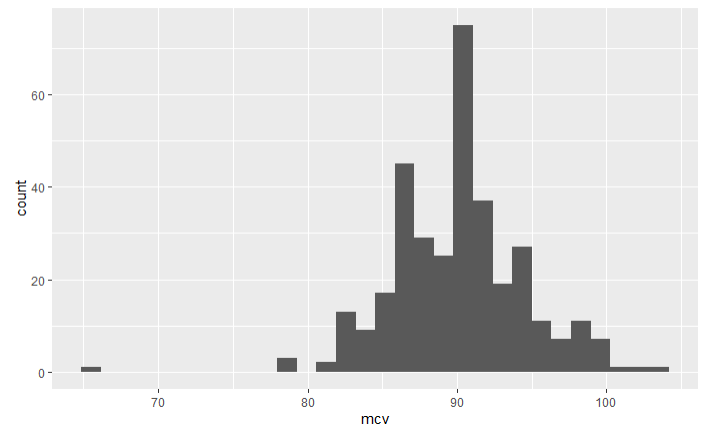
\includegraphics[width=0.7\linewidth]{figures/hist_1}
	\caption{Histograma mcv}
	\label{fig:hist1}
\end{figure}


Se estudia la posibilidad de que los datos sigan una distribución normal a través del test Shapiro-Wilk, no obstante el p-value resultante no supera el nivel de significancia definido en 0.05, por lo que rechazamos la hipótesis nula y negamos una distribución Normal.\\



	
	\item \textbf{alkphos}: 
	\begin{table}[h!]
		\centering
		\begin{tabular}{ll}
			& alkphos    \\
			Valor mínimo            & 23.00      \\
			Primer cuartil          & 57.00      \\
			Mediana                 & 67.00      \\
			Media                   & 69.89      \\
			Tercer cuartil          & 80.00      \\
			Valor máximo            & 138.00     \\ \hline
			Desviación estandar     & 18.4319883 \\ \hline
			Coeficiente de skewness & 0.7457300  \\
			Coeficiente de Kurtosis & 3.690844  
		\end{tabular}
	\end{table}

El dominio de esta variable se halla en el intervalo [23, 138]. Se aprecia una leve desplazamiento del centro de la distribución hacia la izquierda presentando cierta dispersión de los datos respecto este centro. 
\newpage
\begin{figure}[h!]
	\centering
	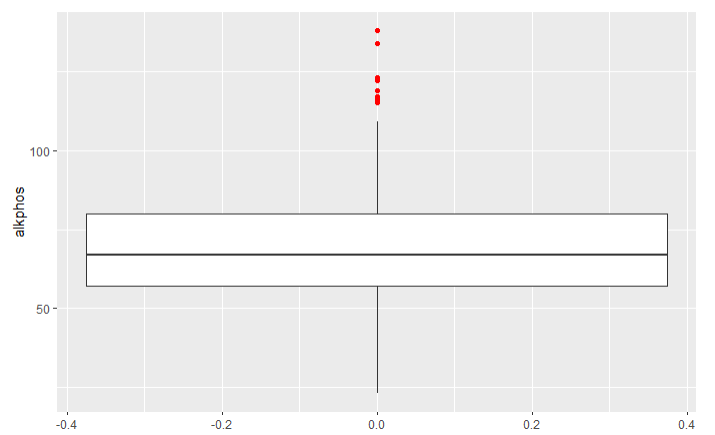
\includegraphics[width=0.7\linewidth]{figures/box_2}
	\caption{Diagrama de cajas alkphos}
	\label{fig:box2}
\end{figure}

\begin{figure}[h!]
	\centering
	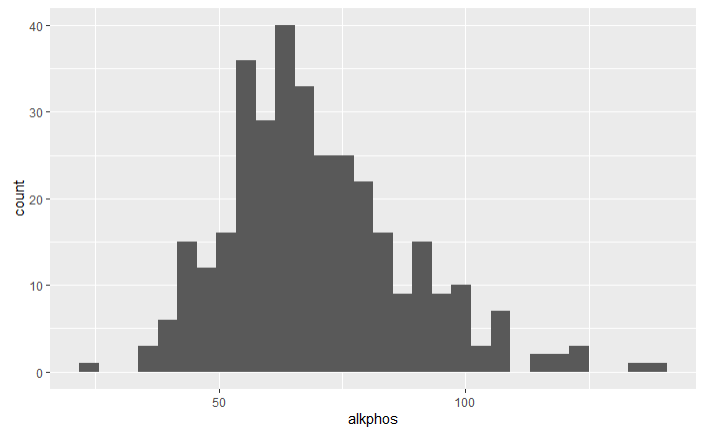
\includegraphics[width=0.7\linewidth]{figures/hist_2}
	\caption{Histograma alkphos}
	\label{fig:hist2}
\end{figure}

De nuevo la distribución se asemeja a una distribución normal, por ello una vez más con el uso del test de Shapiro-Wilk confirmamos un rechazo de la hipótesis nulas, por lo que se niega que la distribución sea normal.\\
	
	\newpage
	\item \textbf{sgpt}: 
	\begin{table}[h!]
		\centering
		\begin{tabular}{ll}
			& sgpt       \\
			Valor mínimo            & 4.00       \\
			Primer cuartil          & 19.00      \\
			Mediana                 & 26.00      \\
			Media                   & 30.51      \\
			Tercer cuartil          & 34.00      \\
			Valor máximo            & 155.00     \\ \hline
			Desviación estandar     & 19.5862490 \\ \hline
			Coeficiente de skewness & 3.0385262  \\
			Coeficiente de Kurtosis & 16.470290 
		\end{tabular}
	\end{table}
	
La variable tratada posee un rango de valores dentro del intervalo [4, 155]. Diferente a los casos anteriores, esta vez se observa una destacable distribución de los datos respecto el centro de la distribución, el cual se sitúa desplazado a la izquierda. Podemos asumir una elevada presencia de outliers a la derecha.

\begin{figure}[h!]
	\centering
	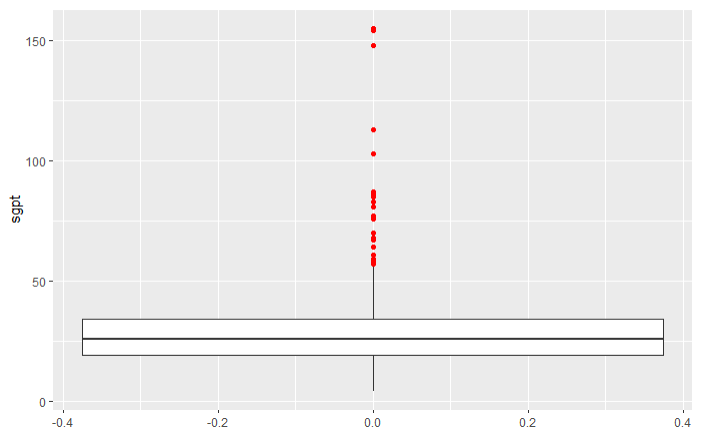
\includegraphics[width=0.7\linewidth]{figures/box_3}
	\caption{Diagrama de cajas sgpt} 
	\label{fig:box3}
\end{figure}
\newpage
\begin{figure}[h!]
	\centering
	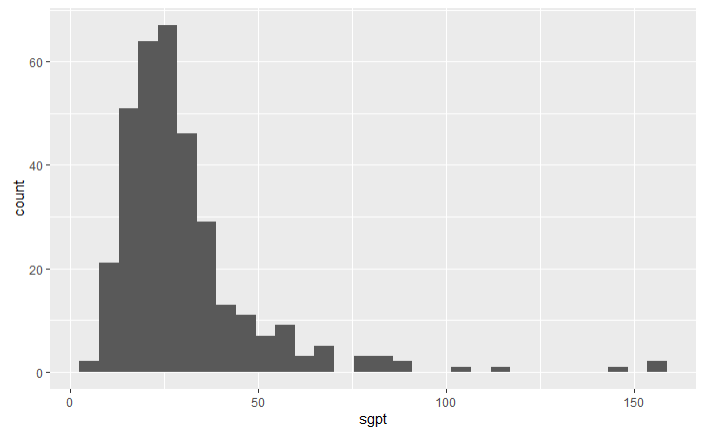
\includegraphics[width=0.7\linewidth]{figures/hist_3}
	\caption{Histograma sgpt}
	\label{fig:hist3}
\end{figure}

En este caso a simple vista podemos confirmar que los datos no presenta una distribución normal, lo cual es confirmado por el test Shapiro-Wilk.\\
	
	\item \textbf{sgot}: 
	\begin{table}[h!]
		\centering
		\begin{tabular}{ll}
			& sgot       \\
			Valor mínimo            & 5.00       \\
			Primer cuartil          & 19.00      \\
			Mediana                 & 23.00      \\
			Media                   & 24.66      \\
			Tercer cuartil          & 27.00      \\
			Valor máximo            & 82.00      \\ \hline
			Desviación estandar     & 10.1155409 \\ \hline
			Coeficiente de skewness & 2.2703414  \\
			Coeficiente de Kurtosis & 10.894188 
		\end{tabular}
	\end{table}
	
	Con un dominio dentro del intervalo [5, 82], esta variable presenta un comportamiento similar a la anterior. Un centro de la distribución desplazado ligeramente a la izquierda con una alta dispersión en los datos, lo cual de nuevo dará lugar a una presencia de outliers a la derecha del centro de la distribución.

	\newpage
\begin{figure}[h!]
	\centering
	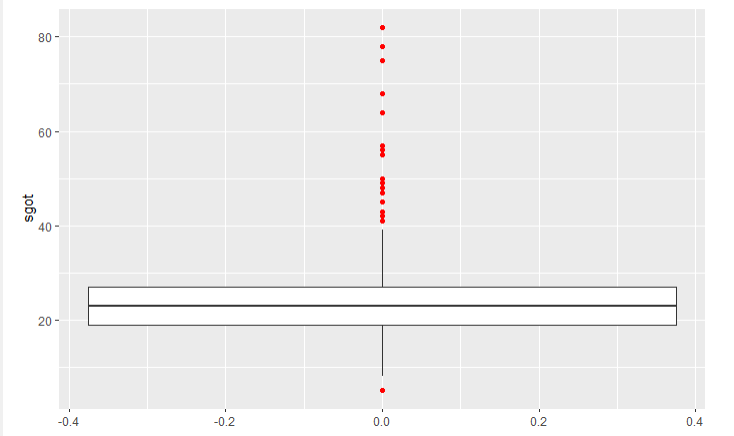
\includegraphics[width=0.7\linewidth]{figures/box_4}
	\caption{Diagrama de cajas sgot}
	\label{fig:box4}
\end{figure}

\begin{figure}[h!]
	\centering
	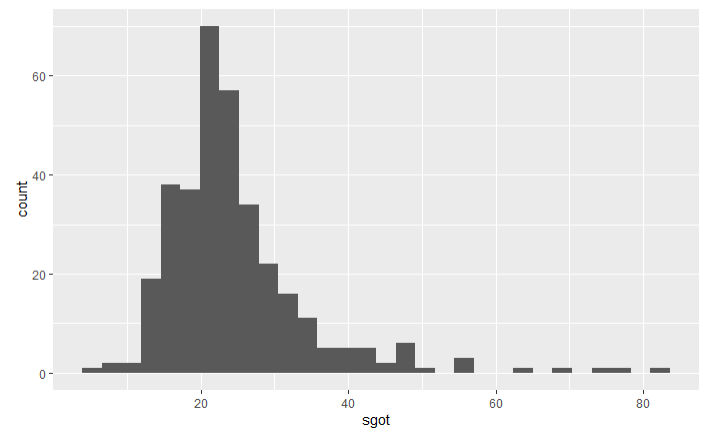
\includegraphics[width=0.7\linewidth]{figures/hist_4}
	\caption{Histograma sgot}
	\label{fig:hist4}
\end{figure}
	
	De nuevo nos alejamos de una distribución normal de los datos.
	
\newpage
	\item \textbf{gammagt}: 
	\begin{table}[h!]
		\centering
		\begin{tabular}{ll}
			& gammagt    \\
			Valor mínimo            & 5.0        \\
			Primer cuartil          & 15.0       \\
			Mediana                 & 25.0       \\
			Media                   & 38.4       \\
			Tercer cuartil          & 46.0       \\
			Valor máximo            & 297.0      \\ \hline
			Desviación estandar     & 39.4393786 \\ \hline
			Coeficiente de skewness & 2.8387489  \\
			Coeficiente de Kurtosis & 13.180100 
		\end{tabular}
	\end{table}
	
	La variable tratada posee los datos dentro del rango [5, 297]. De nuevo un ligero desplazamiento del centro de la distribución a la izquierda junto con una dispersión de estos valores. Se asume una vez más la presencia de outliers a la derecha del centro.
	
\begin{figure}[h!]
	\centering
	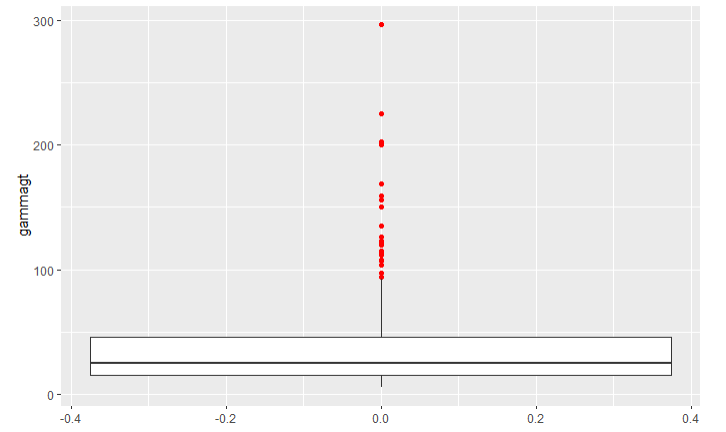
\includegraphics[width=0.7\linewidth]{figures/box_5}
	\caption{Diagrama de cajas gammagt}
	\label{fig:box5}
\end{figure}
\newpage

\begin{figure}[h!]
	\centering
	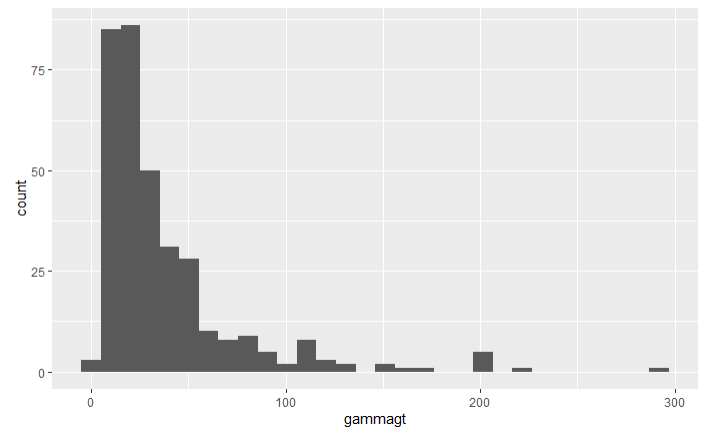
\includegraphics[width=0.7\linewidth]{figures/hist_5}
	\caption{Histograma gammagt}
	\label{fig:hist5}
\end{figure}
	
	Se descarta una distribución normal.
	
	\item \textbf{selector}: 
	Esta variable no merece de estudio profundo pues valdrá 1 o 2 según el dato pertenezca al conjunto de entrenamiento o test.

	
	
\end{itemize}



\subsection{Análisis de las variable dependiente}\label{drinks}
Finalicemos analizando la variable dependiente, \textbf{drinks}:
\begin{table}[h!]
	\centering
	\begin{tabular}{ll}
		& drinks    \\
		Valor mínimo            & 0.000     \\
		Primer cuartil          & 0.500     \\
		Mediana                 & 3.000     \\
		Media                   & 3.431     \\
		Tercer cuartil          & 5.000     \\
		Valor máximo            & 20.000    \\ \hline
		Desviación estandar     & 3.3416404 \\ \hline
		Coeficiente de skewness & 1.5616997 \\
		Coeficiente de Kurtosis & 6.673044 
	\end{tabular}
\end{table}
\newpage
\begin{figure}[h!]
	\centering
	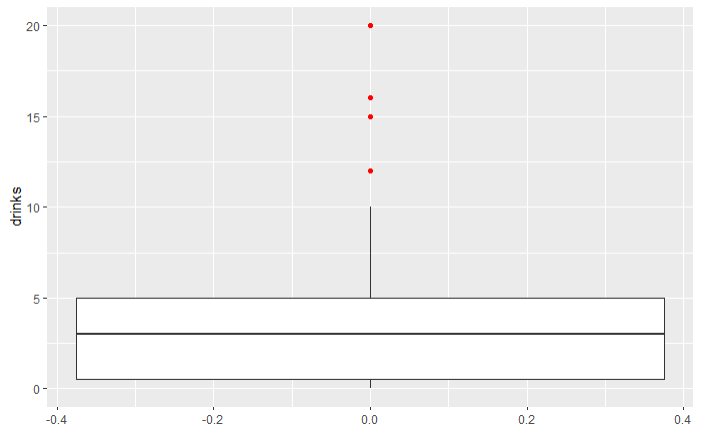
\includegraphics[width=0.7\linewidth]{figures/box_6}
	\caption{Diagrama de cajas drinks}
	\label{fig:box6}
\end{figure}

\begin{figure}[h!]
	\centering
	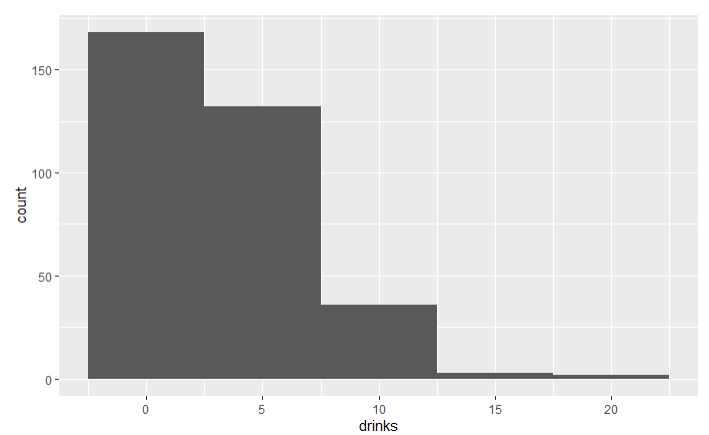
\includegraphics[width=0.7\linewidth]{figures/hist_6}
	\caption{Histograma drinks}
	\label{fig:hist6}
\end{figure}

Se presenta un problema con la variable dependiente, pues existen 16 posibles clases diferentes. Para un modelo de clasificación sobre un dataset este es un valor de clases muy elevado, por ello, tras un proceso de documentación, varios artículos coinciden en separar la variable dependiente en dos posibles valores dependiendo si el valor de drinks $ > $  5. \cite{1}
Siguiendo esta idea y separando los datos según la variable 'selector', la nueva variable drinks contiene:
\begin{table}[h!]
	\centering
	\begin{tabular}{l|ll}
		& selector == 1 & selector == 2 \\ \hline
		drinks \textless{}= 5 & 100           & 157           \\
		drinks \textgreater 5 & 45            & 43           
	\end{tabular}
\end{table}

Se observa un desnivel de casos, algo que se podría solucionar si en lugar de drinks $ > $ 5, se toman aquellas drinks $ > $  3 como punto de separación. Estos nos permitiría obtener dos clases con un número similar de casos, sin embargo sería una separación artificial. Según la información encontrada, tomar menos de 5.5 pintas de medía al día tiene efectos muy bajos en la posibilidad de problemas en el hígado. Mientras que beber por encima de esta cantidad si suele estar vinculado a problemas en el hígado. \cite{2}
Por este motivo considero mejor opción tomar drinks $ > $  5 como separación en dos posibles clases. De esta forma se ha reducido el número de clases de la variable drinks a 2, tomando un valor de 0 si drinks $ \leq $ 5 y un valor de 1 si drinks $ > $ 5.




\vspace{1cm}
\subsection{Análisis de valores anómalos}
Durante el estudio de las variables se han detectado varios casos en los que la presencia de valores anómalos debe ser considerada y estudiada. \\


Respecto a los outliers situados a la izquierda:


\begin{figure}[!tbh]
	\centering
	\begin{subfigure}{0.5\textwidth}
	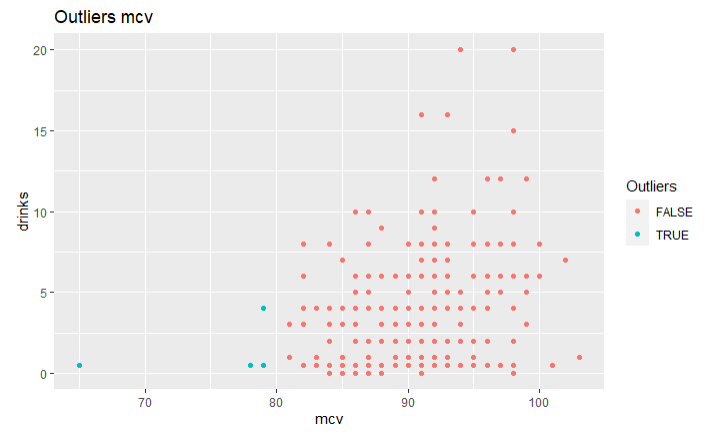
\includegraphics[width=1\linewidth]{figures/outlier_1}
\caption{}
\label{fig:outlier1}
	\end{subfigure}\hfil % <-- added
	\begin{subfigure}{0.5\textwidth}
	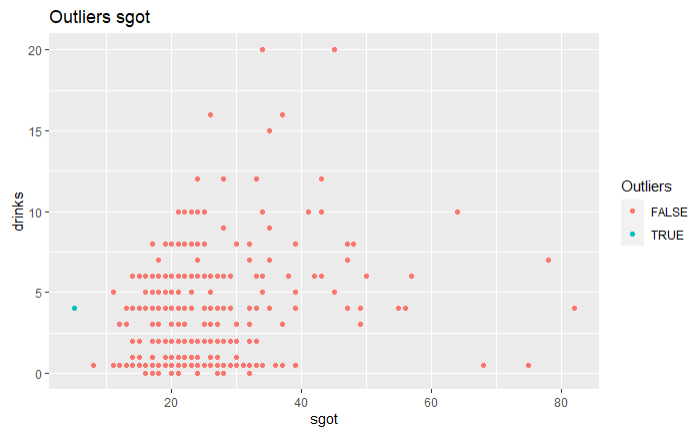
\includegraphics[width=1\linewidth]{figures/outlier_2}
\caption{}
\label{fig:outlier2}
	\end{subfigure}\hfil % <-- added
\end{figure}



\newpage
Respecto a los outliers situados a la derecha:
\begin{figure}[!tbh]
	\centering
	\begin{subfigure}{0.5\textwidth}
	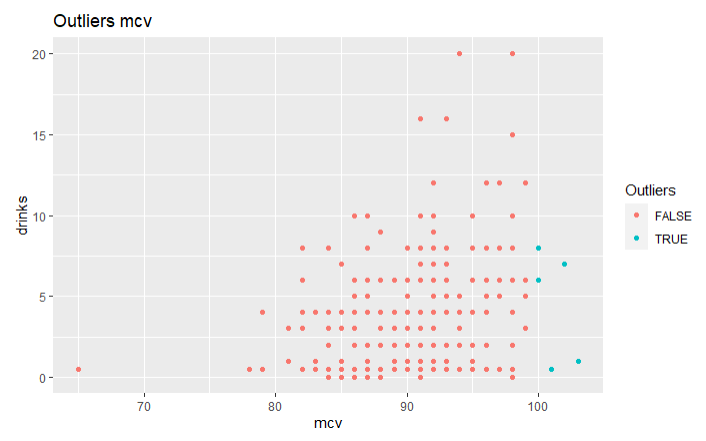
\includegraphics[width=1\linewidth]{figures/outlier_3}
\caption{}
\label{fig:outlier3}
	\end{subfigure}\hfil % <-- added
	\begin{subfigure}{0.5\textwidth}
	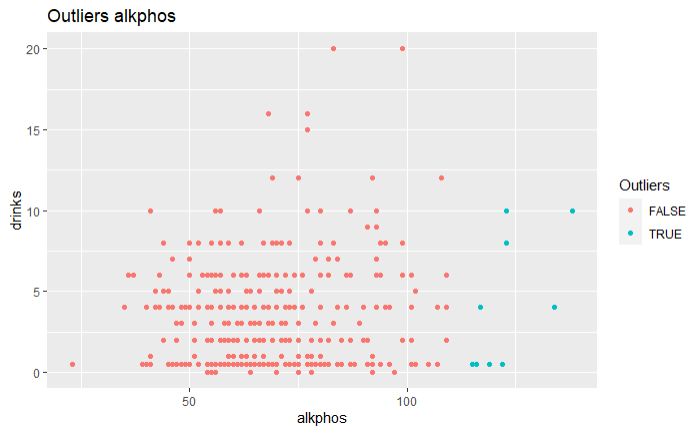
\includegraphics[width=1\linewidth]{figures/outlier_4}
\caption{}
\label{fig:outlier4}
	\end{subfigure}\hfil % <-- added
	
	\medskip
	
	\begin{subfigure}{0.5\textwidth}
	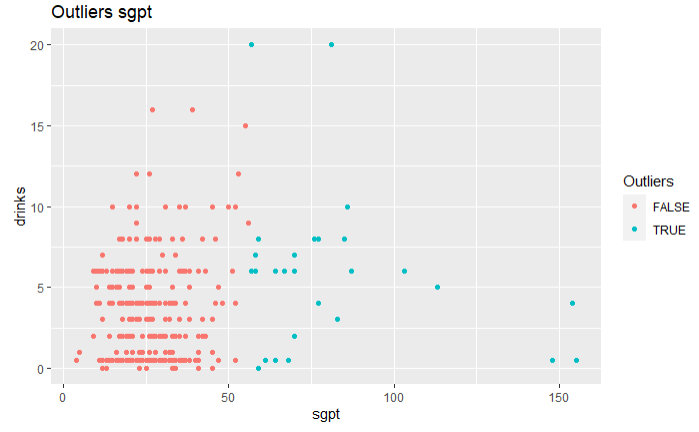
\includegraphics[width=1\linewidth]{figures/outlier_5}
\caption{}
\label{fig:outlier5}
	\end{subfigure}\hfil % <-- added
	\begin{subfigure}{0.5\textwidth}
	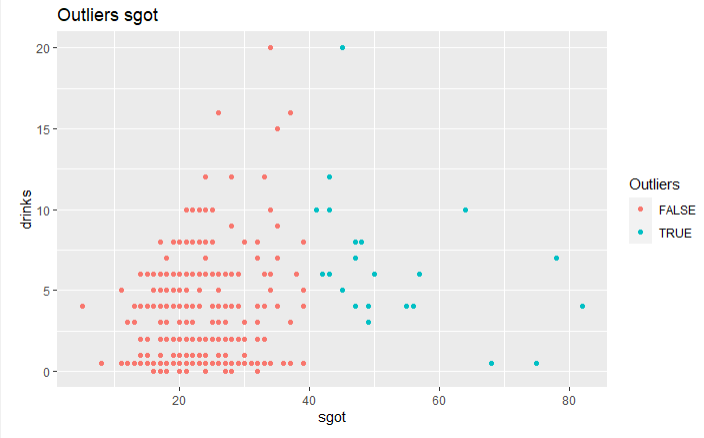
\includegraphics[width=1\linewidth]{figures/outlier_6}
\caption{}
\label{fig:outlier6}
	\end{subfigure}\hfil % <-- added
	
	\medskip
	\begin{subfigure}{0.5\textwidth}
		\centering
	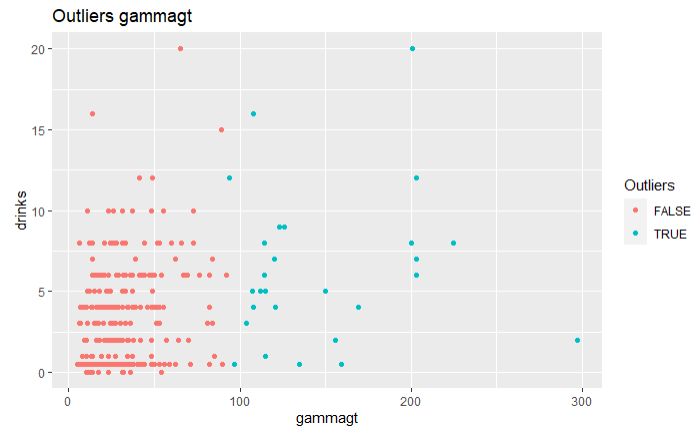
\includegraphics[width=1\linewidth]{figures/outlier_7}
\caption{}
\label{fig:outlier7}
	\end{subfigure}\hfil % <-- added
	
	\caption{Outliers Bupa}
	\label{out}
\end{figure}





En casos como la variable 'sgpt' se observa que la presencia de outliers se debe a que los datos poseen una alta concentración en una zona en concreto. Pese a la existencia de estos casos con valores extremos, considero que su eliminación sería un error. En primer lugar tratamos con un dataset muy pequeño, por lo tanto la eliminación de casos será notable. Por otra parte, el estudio de casos donde los diferentes test de análisis de sangre han obtenido resultados elevados puede ser muy importante para definir casos en los que el consumo de alcohol es elevado y por tanto las posibilidades de una enfermedad de hígado son mayores.



\newpage
\section{Análisis de las relaciones entre variables}
Analizada las distribuciones de las diferentes variables que forman este dataset, se procede en esat sección al análisis de las posibles relaciones existentes entre las mismas, con el objetivo de determinar la posible existencia de relaciones entre variables, detalle a tener en cuenta en el posterior proceso de elaboración de modelos.\\

El siguiente diagrama de correlaciones permite efectuar este estudio entre cada par de variables que forman el dataset, realizando el calculo de las correlaciones mediante el test de Kendall. Se han excluido la variable 'selector' y 'drinks' para esta representación, pues es evidente que no aportarán información útil. 

\begin{figure}[!h]
	\centering
	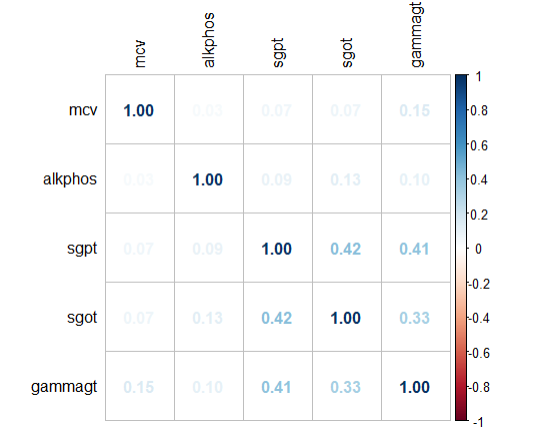
\includegraphics[width=0.7\linewidth]{figures/corr_2}
	\caption{}
	\label{fig:corr2}
\end{figure}

Observamos que unicamente destacan dos relaciones, la correlación positiva entre 'sgpt' - 'sgot' y  'sgpt' - 'gammagt'. Esta relación nos indica que estos test de análisis de sangre poseen unas métricas similares, y que por lo tanto, los resultados de estos poseen valores similares. Pese a ello la relación no es lo suficientemente fuerte como para ser altamente considerable. Esta posible relación será tratada en la siguiente sección.







\newpage
\section{Comprobación de hipótesis planteadas}
\textbf{Una mayor masa corporal puede dar lugar a casos en los que un alto consumo de alcohol no se vincule con altos resultados en los análisis de sangre.}
	 
Recordando que un valor drinks de 1 significa que el consumo está por encima del recomendado, y por tanto se clasifica como muy posible problema en el hígado, mientras que un valor de drinks de 0 indica un bajo consumo y menor posibilidad de enfermedad, nos apoyamos en las siguientes gráficas:


\begin{figure}[!tbh]
	\centering
	\begin{subfigure}{0.5\textwidth}
	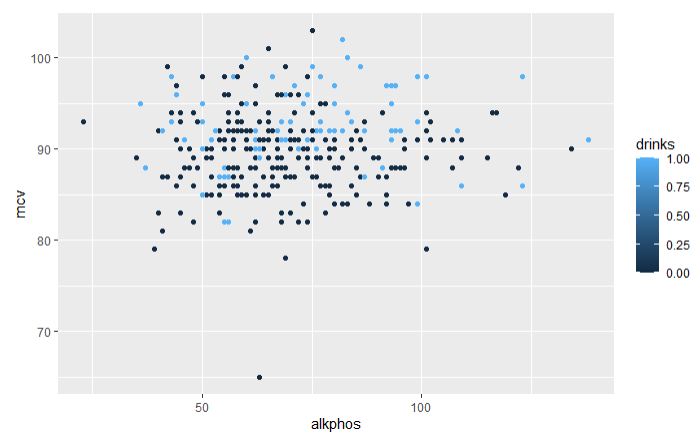
\includegraphics[width=1\linewidth]{figures/tesis_1}
\caption{}
\label{fig:tesis1}
	\end{subfigure}\hfil % <-- added
	\begin{subfigure}{0.5\textwidth}
	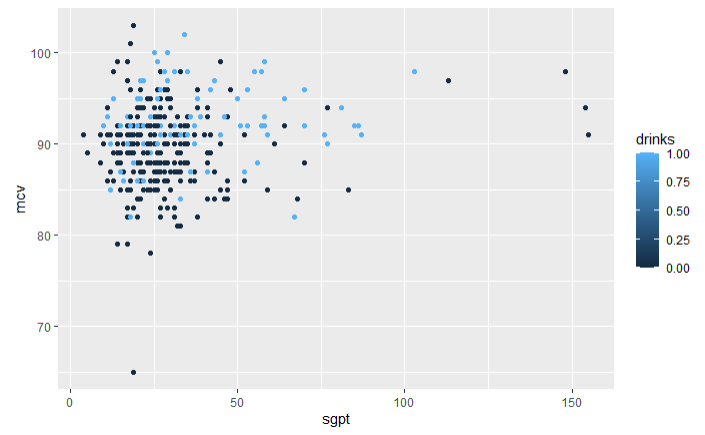
\includegraphics[width=1\linewidth]{figures/tesis_2}
\caption{}
\label{fig:tesis2}
	\end{subfigure}\hfil % <-- added
	
	\medskip
	
	\begin{subfigure}{0.5\textwidth}
	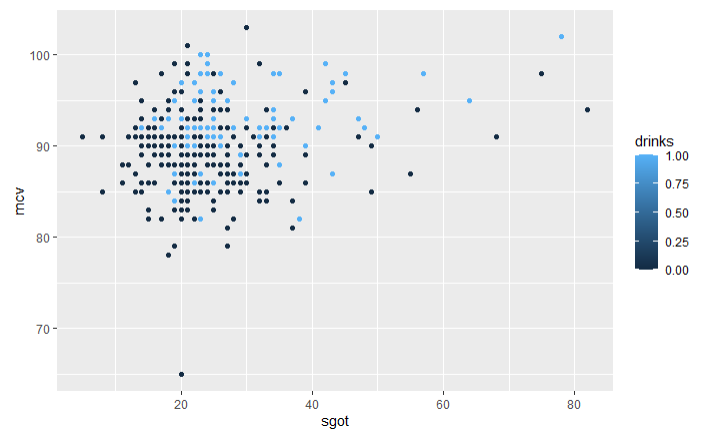
\includegraphics[width=1\linewidth]{figures/tesis_3}
\caption{}
\label{fig:tesis3}
	\end{subfigure}\hfil % <-- added
	\begin{subfigure}{0.5\textwidth}
	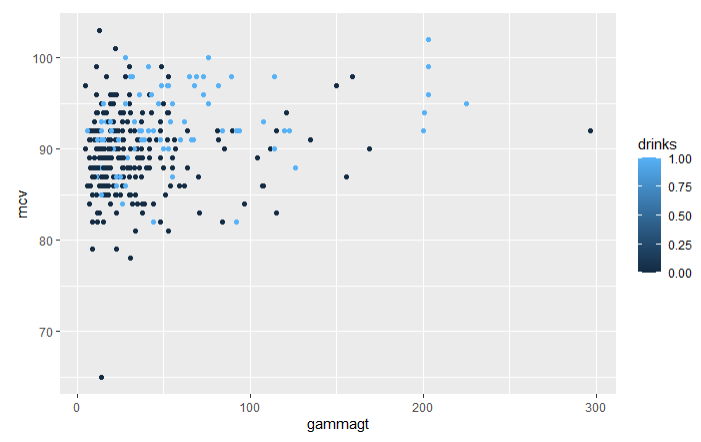
\includegraphics[width=1\linewidth]{figures/tesis_4}
\caption{}
\label{fig:tesis4}
	\end{subfigure}\hfil % <-- added
	
	\caption{Hipótesis 1}
	\label{hipo1}
\end{figure}




Se observa que en varios casos con alta masa corporal (mcv), un considerado alto consumo de alcohol (drinks=1) no se vincula con un alto valor en los resultados del test de análisis de sangre, confirmando la hipótesis planteada.\\

 De este punto se pueden sacar varias conclusiones. La primera es que la masa corporal será de importancia en el desarrollo de correctos modelos de clasificación. Por otra parte, la detección de un alto consumo de alcohol no será posible con un único análisis de sangre, siendo importante la combinación de los cuatro diferentes análisis presentes en el dataset. 
	
\newpage
\textbf{¿Un valor alto en uno de los test de análisis de sangre equivale a un valor alto en el resto de test?}	 

Es cierto que para todas las variables que representan os resultados de un test de sangre, un valor elevado significa una mayor probabilidad de tener una enfermedad de hígado. Sin embargo, observando los diferentes dominios presentes en cada una de estas variables se observa que cada una tiene su propia métrica. \\

Para ello comparemos cada análisis de dos en dos:
\begin{figure}[!tbh]
	\centering
	\begin{subfigure}{0.5\textwidth}
	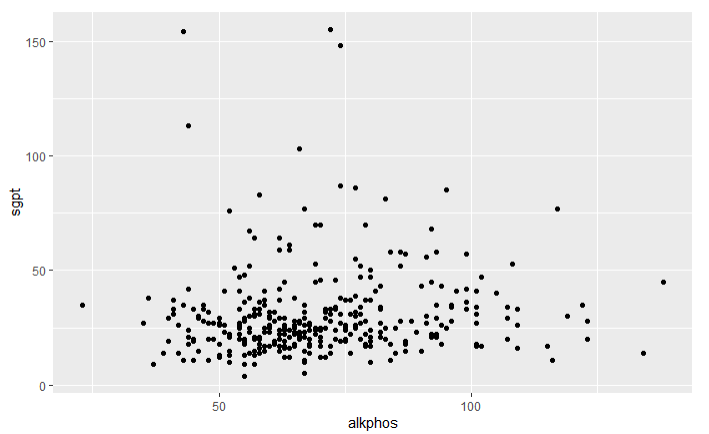
\includegraphics[width=1\linewidth]{figures/tesis_5}
\caption{}
\label{fig:tesis5}
	\end{subfigure}\hfil % <-- added
	\begin{subfigure}{0.5\textwidth}
	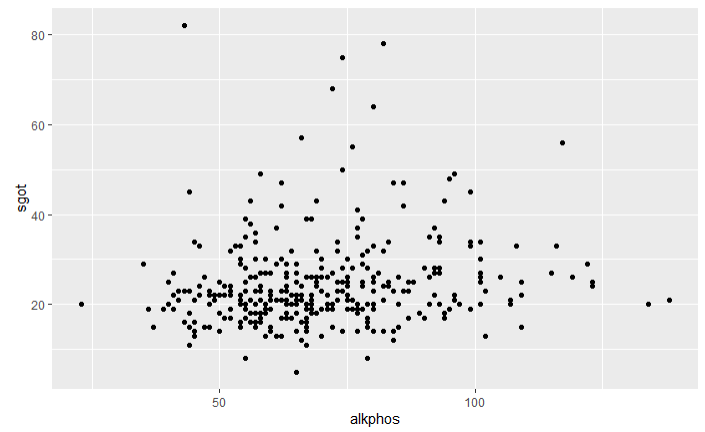
\includegraphics[width=1\linewidth]{figures/tesis_6}
\caption{}
\label{fig:tesis6}
	\end{subfigure}\hfil % <-- added
	
	\medskip
	
	\begin{subfigure}{0.5\textwidth}
	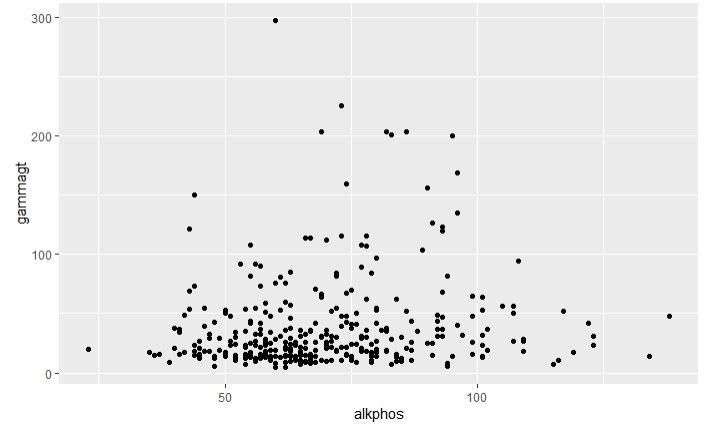
\includegraphics[width=1\linewidth]{figures/tesis_7}
\caption{}
\label{fig:tesis7}
	\end{subfigure}\hfil % <-- added
	\begin{subfigure}{0.5\textwidth}
	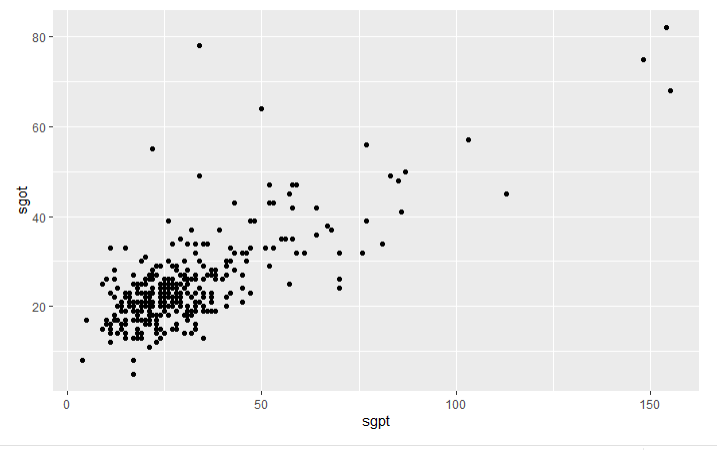
\includegraphics[width=1\linewidth]{figures/tesis_8}
\caption{}
\label{fig:tesis8}
	\end{subfigure}\hfil % <-- added

	\medskip

\begin{subfigure}{0.5\textwidth}
	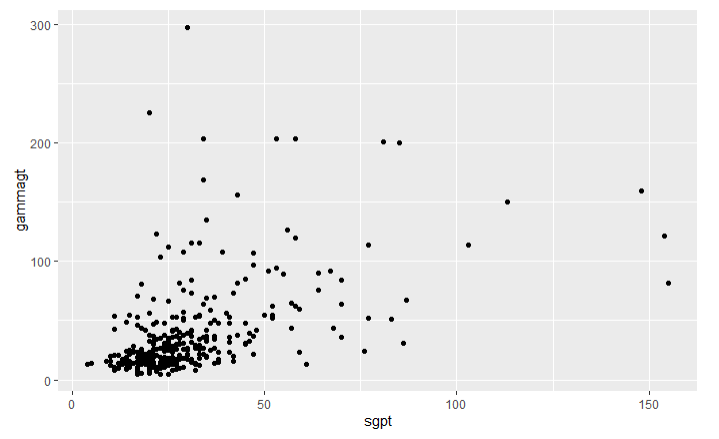
\includegraphics[width=1\linewidth]{figures/tesis_9}
	\caption{}
	\label{fig:tesis9}
\end{subfigure}\hfil % <-- added
\begin{subfigure}{0.5\textwidth}
	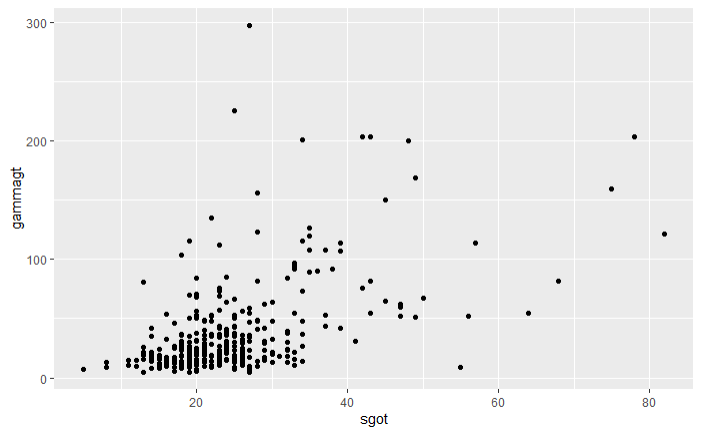
\includegraphics[width=1\linewidth]{figures/tesis_10}
	\caption{}
	\label{fig:tesis10}
\end{subfigure}\hfil % <-- added
	
	\caption{Hipótesis 2}
	\label{hipo2}
\end{figure}



En la mayoría de los casos se observa que un resultado elevado en uno de los test de sangre no significa que en los demás se obtenga un valor también elevado. El único caso en el que un valor alto en ese test de sangre equivale a un valor alto en otro test es en la relación entre 'sgot' y 'sgpt'.
	



